\documentclass[a4paper,12pt]{article}
\usepackage[utf8]{inputenc} 
\usepackage{hyperref}
\usepackage{geometry}
\geometry{a4paper, margin=1in}
\usepackage{graphicx} 
\usepackage{enumitem}
\usepackage{graphicx,url}
\usepackage[english,portuguese]{babel}
\usepackage{sbc-template}
\usepackage{amsmath}

\geometry{a4paper, margin=1in}

\begin{document}
\begin{center}
\LARGE \textbf{Computação, Sociedade e Sustentabilidade\\Componente Educacional} \\
\normalsize

\vspace{1cm}

Nunno Wakiyama\inst{1}, Pedro Victor Luna\inst{2}, Victor Vilela\inst{3} e Rodrigo Diniz\inst{4} \\

\vspace{1cm}

ICAM - C3 -- Universidade Católica de Pernambuco (UNICAP) \\

Caixa Postal 526 -- 50.050-900 -- Recife -- PE -- Brasil \\

\vspace{1cm}

\small{
\href{mailto:Nunno000000849115@unicap.br}{Nunno000000849115@unicap.br}, 
\href{mailto:pedro000000851061@unicap.br}{pedro000000851061@unicap.br}, 
\href{mailto:victor000000850712@unicap.br}{victor000000850712@unicap.br}, 
\href{mailto:rodrigo000000851563@unicap.br}{rodrigo000000851563@unicap.br}
}
\end{center}
\normalsize

\vspace{2cm}

\large
\section{\LARGE{Resumo e Abstract}}

\vspace{0.5cm}

\selectlanguage{portuguese}

\begin{resumo}
Resumo. Este artigo tem como objetivo apresentar, de maneira concisa, o processo de execução do componente educacional do nosso projeto final na disciplina de Computação, Sociedade e Sustentabilidade. Esse componente foi direcionado às crianças que frequentam a biblioteca dos Tabaiares e consistiu em demonstrar, por meio de atividades lúdicas, diversas formas de se divertir e aprender coisas novas de maneira saudável e interativa. 
\end{resumo}

\selectlanguage{english}

\begin{abstract}
Abstract. This article aims to concisely present the process of implementing the educational component of our final project in the discipline of Computing, Society and Sustainability. This component was aimed at children who frequent the Tabaiares library and consisted of demonstrating, through playful activities, different ways of having fun and learning new things in a healthy and interactive way. 
\end{abstract}
\newpage

\section{\LARGE{Sumário}}
\tableofcontents

\newpage

\section{\LARGE{Introdução}}
\vspace{0.5cm}

\subsection{\Large{Apresentação do tema}}
Qual será o destino da humanidade diante da prevalência das telas e dos vícios na estrutura social contemporânea? Foi deste princípio que partimos para começar os trabalhos da componente educacional do nosso projeto de Computação, Sociedade e Sustentabilidade. O objetivo do grupo era apresentar às crianças que frequentavam a Biblioteca Caranguejo dos Tabaiares que existem formas de aprender com o uso da tecnologia, ao mesmo tempo em que se buscava apresentar alternativas de entretenimento que não se atrelassem exclusivamente à mídia eletrônica.\vspace{0.3cm}\\
Para alcançar tal propósito, empregamos metodologias e plataformas ainda desconhecidas pelo nosso público-alvo no intuito de realmente fazer algo diferente e que chamasse bastante atenção das crianças.
\vspace{0.2cm}

\subsection{\Large{Justificativa}}
Youtube shorts, rells do instagram e os vídeos curtos do tiktok. Estes são os formatos adotados para os vídeos rápidos e concisos nessas plataformas, vídeos que se popularizaram muito no período da pandemia do Covid-19. Ok, mas o que esses 3 exemplos tem em comum? De forma breve, os 3 são exemplos de entretenimento digital que, apesar de sua brevidade e alta consumibilidade, são frequentemente considerados formas fúteis e pouco significativas de passar o tempo na internet, mas o que isso quer dizer? Significa que é uma tecnologia desenvolvida com o objetivo de prender o usuário por longas horas a ponto de nem mesmo o próprio usuário perceber a passagem do tempo. Dessa forma as pessoas vão ficando cada vez mais dependentes e viciadas, muitas vezes nem tendo noção do que está acontecendo em suas vidas e tratando com naturalidade.\vspace{0.3cm}\\
Diante desta problemática, nossa equipe iniciou um processo de reflexão visando desenvolver estratégias para evitar que as novas gerações internalizem esses padrões como normais em suas vidas. Nosso objetivo é garantir que as crianças que frequentam a biblioteca tenham a oportunidade de crescer de maneira saudável, conforme as expectativas comumente estabelecidas.
\vspace{0.2cm}

\newpage

\subsection{\Large{Objetivos}}
Outra questão que merece destaque é que a biblioteca, sob a direção de Reginaldo Pereira, dedica especial atenção ao ensino do francês para as crianças, oferecendo aulas regulares de francês e uma coleção de livros para incentivar o aprendizado. \vspace{0.3cm}\\
Diante da problemática apresentada e das reflexões realizadas, concluímos que, para que as crianças pudessem crescer de forma saudável, não seria suficiente apenas abordar o assunto em questão através de conversas. Assim, partimos do princípio de que ensiná-las a utilizar o tempo de maneira produtiva seria uma abordagem mais eficaz. Nesse sentido, decidimos realizar seis atividades com as crianças. quatro dessas atividades consistiram em oficinas de aprendizagem, incluindo três oficinas de origami e uma oficina de mágica. A quarta atividade envolveu a realização de um jogo no formato de quiz chamado Kahoot, que abordava palavras básicas em francês e países onde o francês é a língua oficial, temas recentemente discutidos nas aulas com as crianças. Finalmente, a última atividade foi uma aula de francês que cobriu tópicos básicos como opostos (por exemplo, grande e pequeno), nomes de animais de estimação (por exemplo, gato e cachorro) e cores (por exemplo, amarelo e verde). Esta aula foi ministrada por um membro do grupo com conhecimento prévio da língua francesa.\\

\section{\LARGE{Materiais e Métodos (ou Metodologia)}}
\vspace{0.5cm}

\subsection{\Large{Métodos (ou Metodologias) usadas}}
Como mencionado anteriormente no tópico "3.3 Objetivos", o nosso propósito, enquanto grupo, era realizar seis atividades, sendo quatro delas em formato de oficina didática de origami e mágica, uma em formato de quiz Kahoot e outra em formato de aula de francês. Nosso intuito era que todas as atividades fossem realizadas com o maior número possível de crianças. Para alcançar esse objetivo, era crucial a presença de todos os membros da equipe educacional em todos os encontros na biblioteca, uma vez que lidar com crianças pequenas não é uma tarefa simples. Tal interação exige muita atenção, paciência, empatia, comunicação clara, entre outras habilidades essenciais.
\newpage
É importante mencionar que realizamos uma visita no dia 27 de março de 2024 para analisar todo o ambiente da biblioteca, tirar fotos e esclarecer algumas dúvidas com o anfitrião, Reginaldo Pereira. Durante essa visita, obtivemos informações sobre a média diária de crianças frequentadoras do local e solicitamos a opinião de Reginaldo sobre nossas propostas.
\vspace{0.2cm}

\subsection{\Large{Datas, Horários e Materiais necessários}}
Tendo em mente nosso objetivo, métodos e metodologias, fatava apenas implementar tudo que havia sido planejado. Sendo assim, agendamos datas e horários para todas as atividades e separamos tudo que seria necessário para realizar as atividades.\vspace{0.2cm}\\

\subsubsection{Datas e Horários}
1.- Quizz kahoot (17/04/2024 - quarta-feira de 9:20h ás 10:20h)\\
2.- Aula de francês (17/04/2024 - quarta-feira de 10:20h ás 11:00h )\\
3.- Oficina de origami encontro 1 (24/04/2024 - quarta-feira de 9:20h ás 10:20h)\\
4.- Oficina de mágica (24/04/2024 - quarta-feira de 10:20h ás 11:00h)\\
5.- Oficina de origami encontro 2 (08/05/2024 - quarta-feira de 9:20h ás 10:20h)\\
6.- Oficina de origami encontro 3 (08/05/2024 - quarta-feira de 10:20h ás 11:00h)

\subsubsection{Materiais necessários}\vspace{0.3cm}
1.- Quizz kahoot (Um quizz no site kahoot.com com perguntas diversas)\\
2.- Aula de francês (Pré-seleção de vídeos para auxiliar e seleção de assuntos)\\
3.- Origami (Papeis coloridos pré-cortados no formato necessário)\\
4.- Mágica (Pelo menos 2 baralhos completos e alguns objetos de mágica)\vspace{0.2cm}\\

\section{\LARGE{Resultados e Discussão}}
\vspace{0.5cm}

\subsection{\Large{Resultados}}
\vspace{0.2cm}
Neste tópico, serão apresentadas fotos e comentários acerca das atividades realizadas pelo grupo.

\subsubsection{Quizz Kahoot}
A atividade foi realizada com êxito, recebendo uma grande aprovação das crianças, que demonstraram entusiasmo e desejaram por mais. O resultado esteve alinhado com a previsão de Reginaldo quando perguntamos sua opinião sobre o evento. Seguem algumas fotos da atividade:

\vspace{1cm}


\href{https://play.kahoot.it/v2/?quizId=28a22c69-5679-45eb-b411-e55ef0a63311}{Kahoot quizz}\\

\begin{figure}[h]
    \centering
    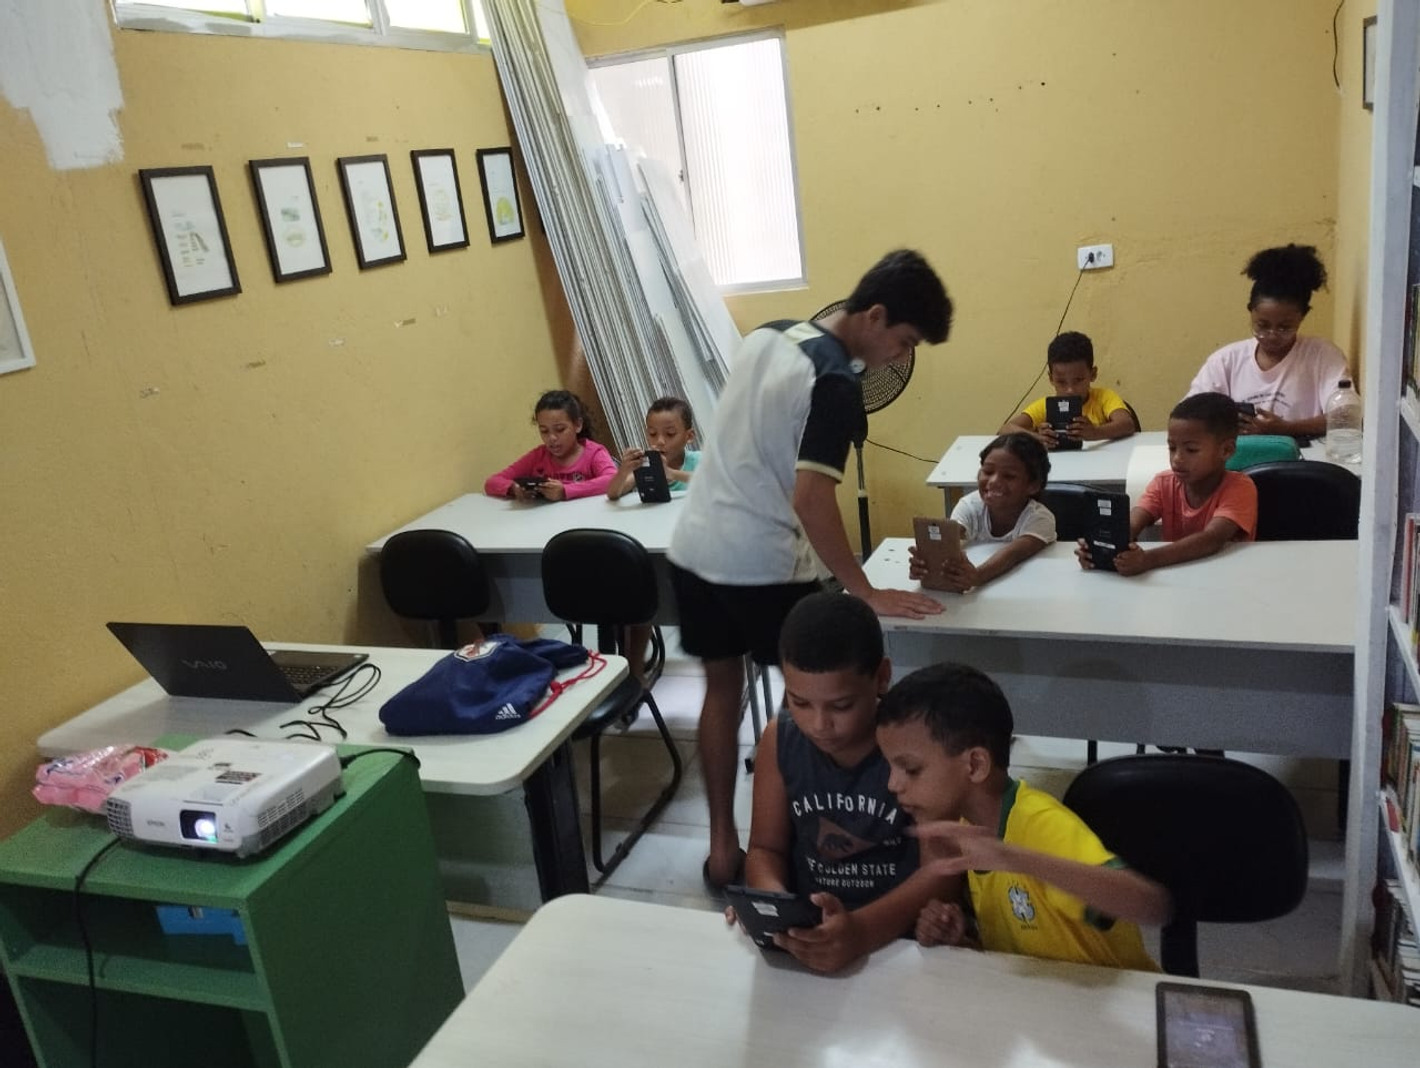
\includegraphics[width=0.5\textwidth]{image.png}
    \caption{Foto 1 das atividades quizz kahoot}
    \label{fig:foto1505}
\end{figure}

\vspace{1cm}

\begin{figure}[h]
    \centering
    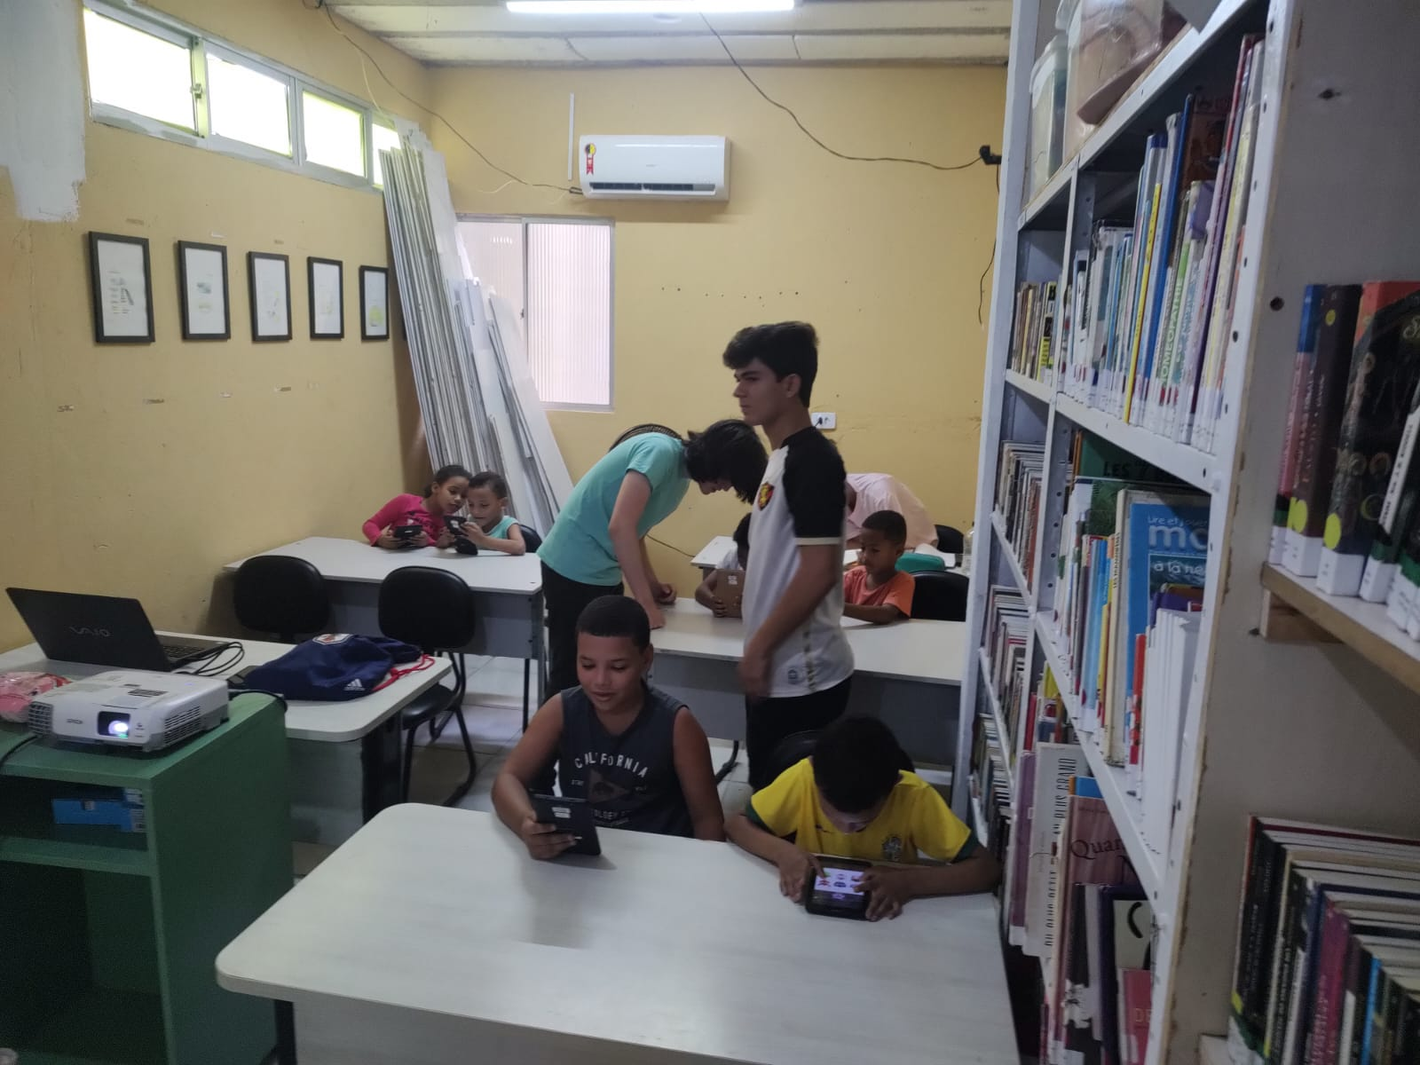
\includegraphics[width=0.5\textwidth]{imagem2.png}
    \caption{Foto 2 das atividades quizz kahoot}
    \label{fig:foto1505}
\end{figure}

\newpage

\subsubsection{Aula de Francês}
Outra atividade realizada com êxito envolveu uma grande interação das crianças, que participaram ativamente da aula, praticando a pronúncia das palavras e fazendo diversas perguntas sempre que surgiam dúvidas. A seguir, apresentamos algumas fotos da atividade:

\vspace{1cm}

\href{https://youtu.be/hx6BJ9j1B3M?si=gRjxKt_P_RIAn7jv}{Vídeo de apoio 1 (Animais de estimação)}\\

\href{https://youtu.be/DAjssWEquzM?si=hfMAgDxSrmBPtaai}{Vídeo de apoio 2 (Cores)}\\

\href{https://youtu.be/mGy9uM4Dk8E?si=Gd58lWWFJuV8rbko}{Vídeo de apoio 3 (Opostos)}\\

\begin{figure}[h]
    \centering
    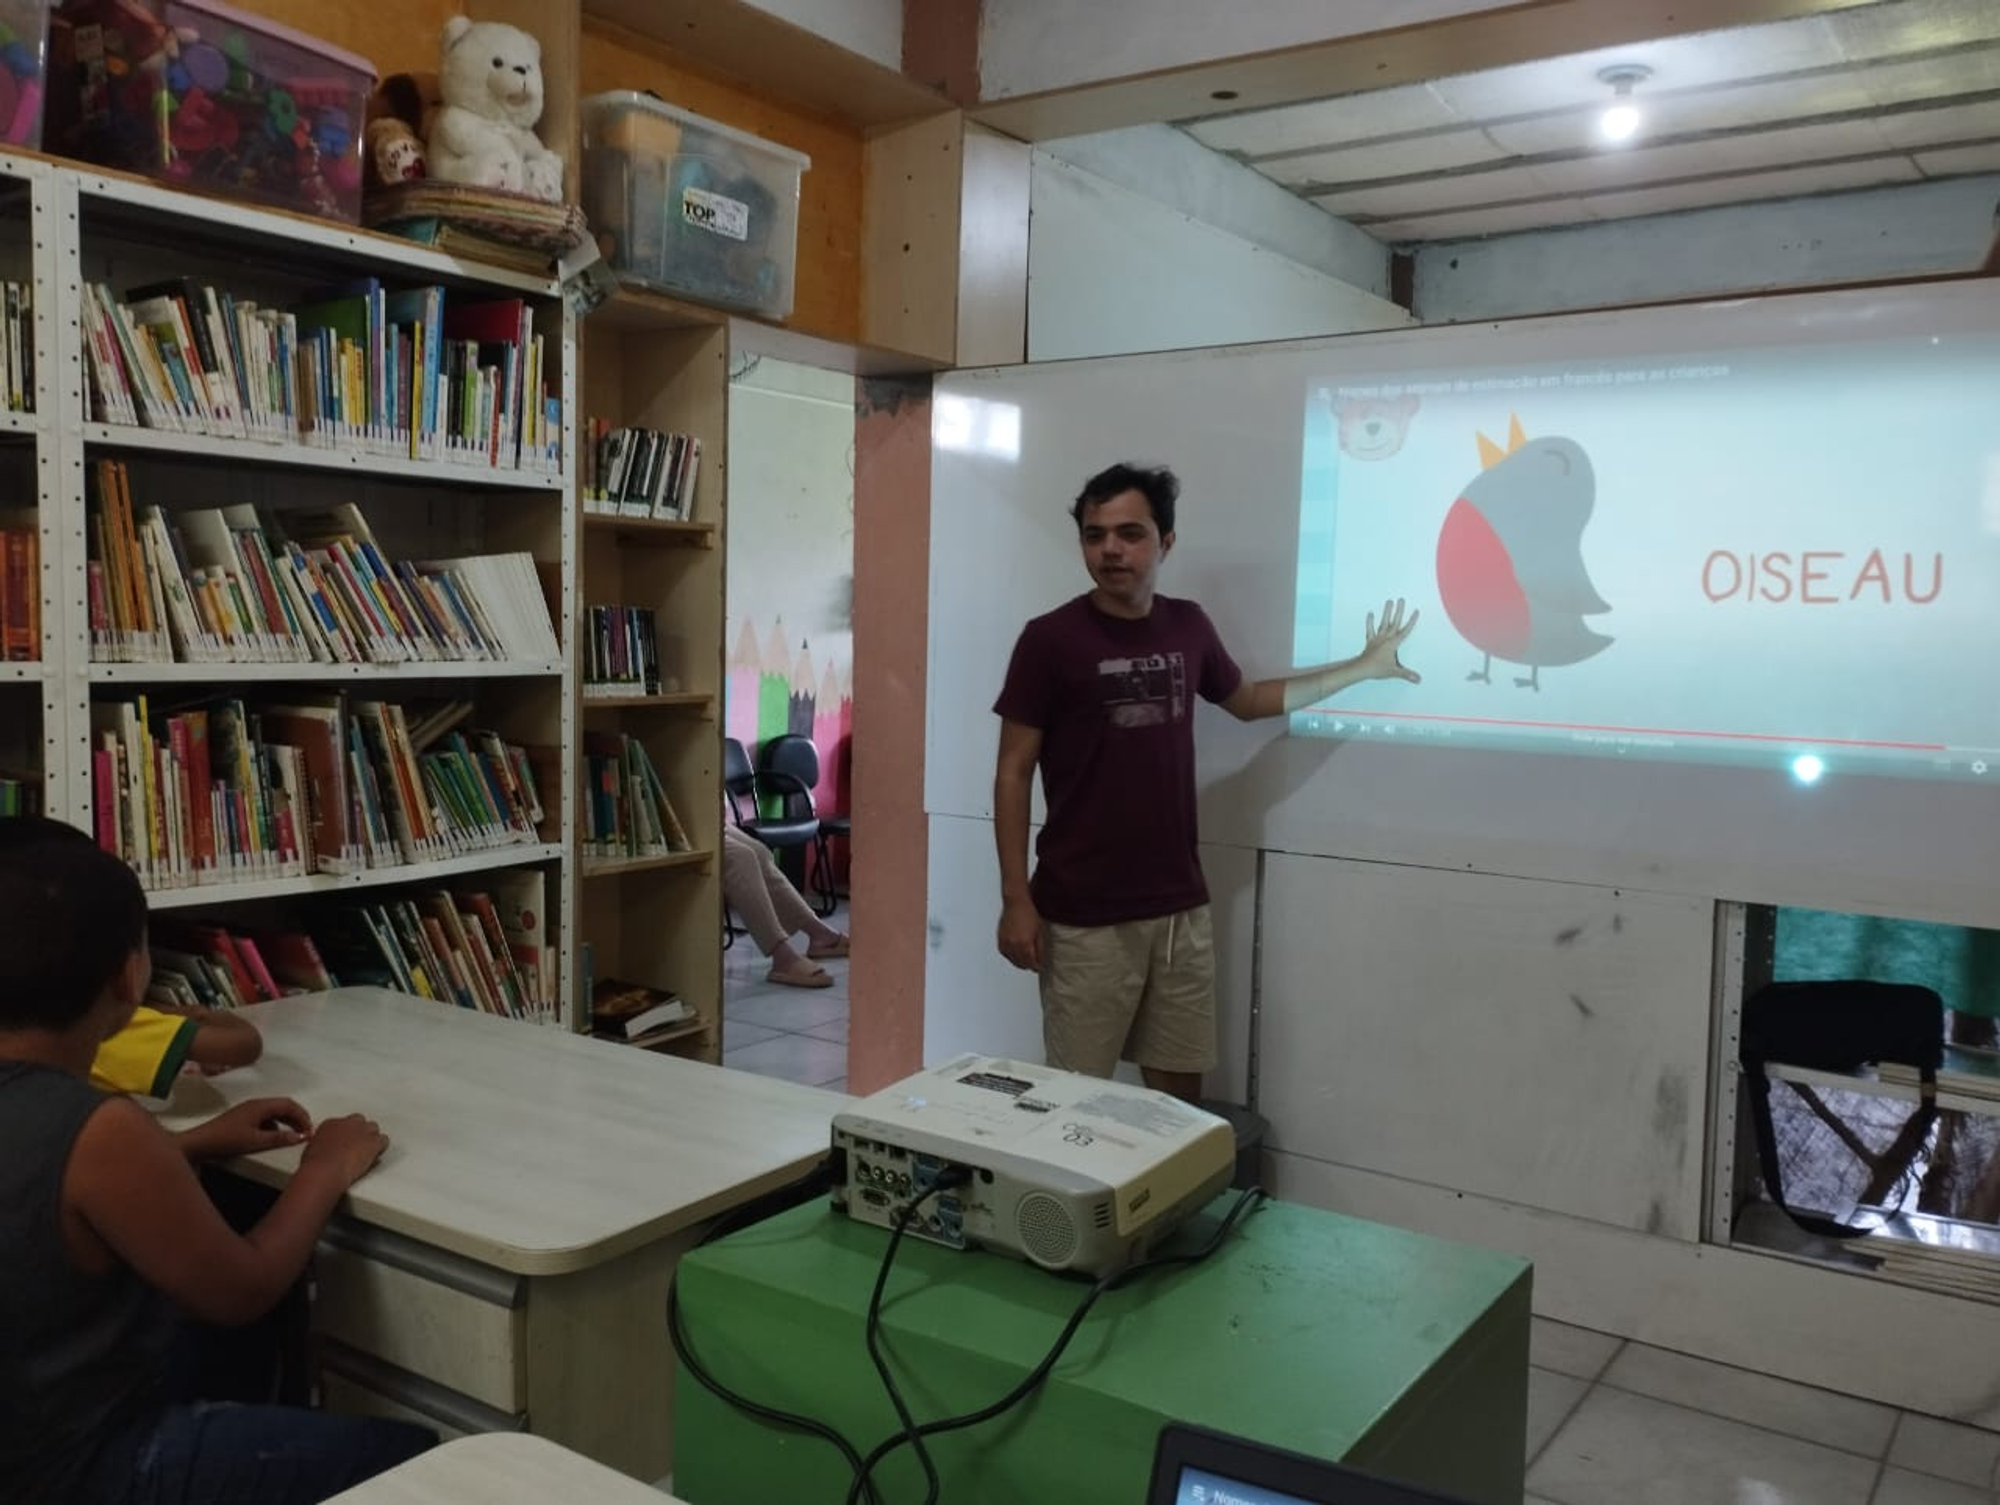
\includegraphics[width=0.5\textwidth]{imagem4.png}
    \caption{Foto 1 aula de francês}
    \label{fig:foto1505}
\end{figure}

\begin{figure}[h]
    \centering
    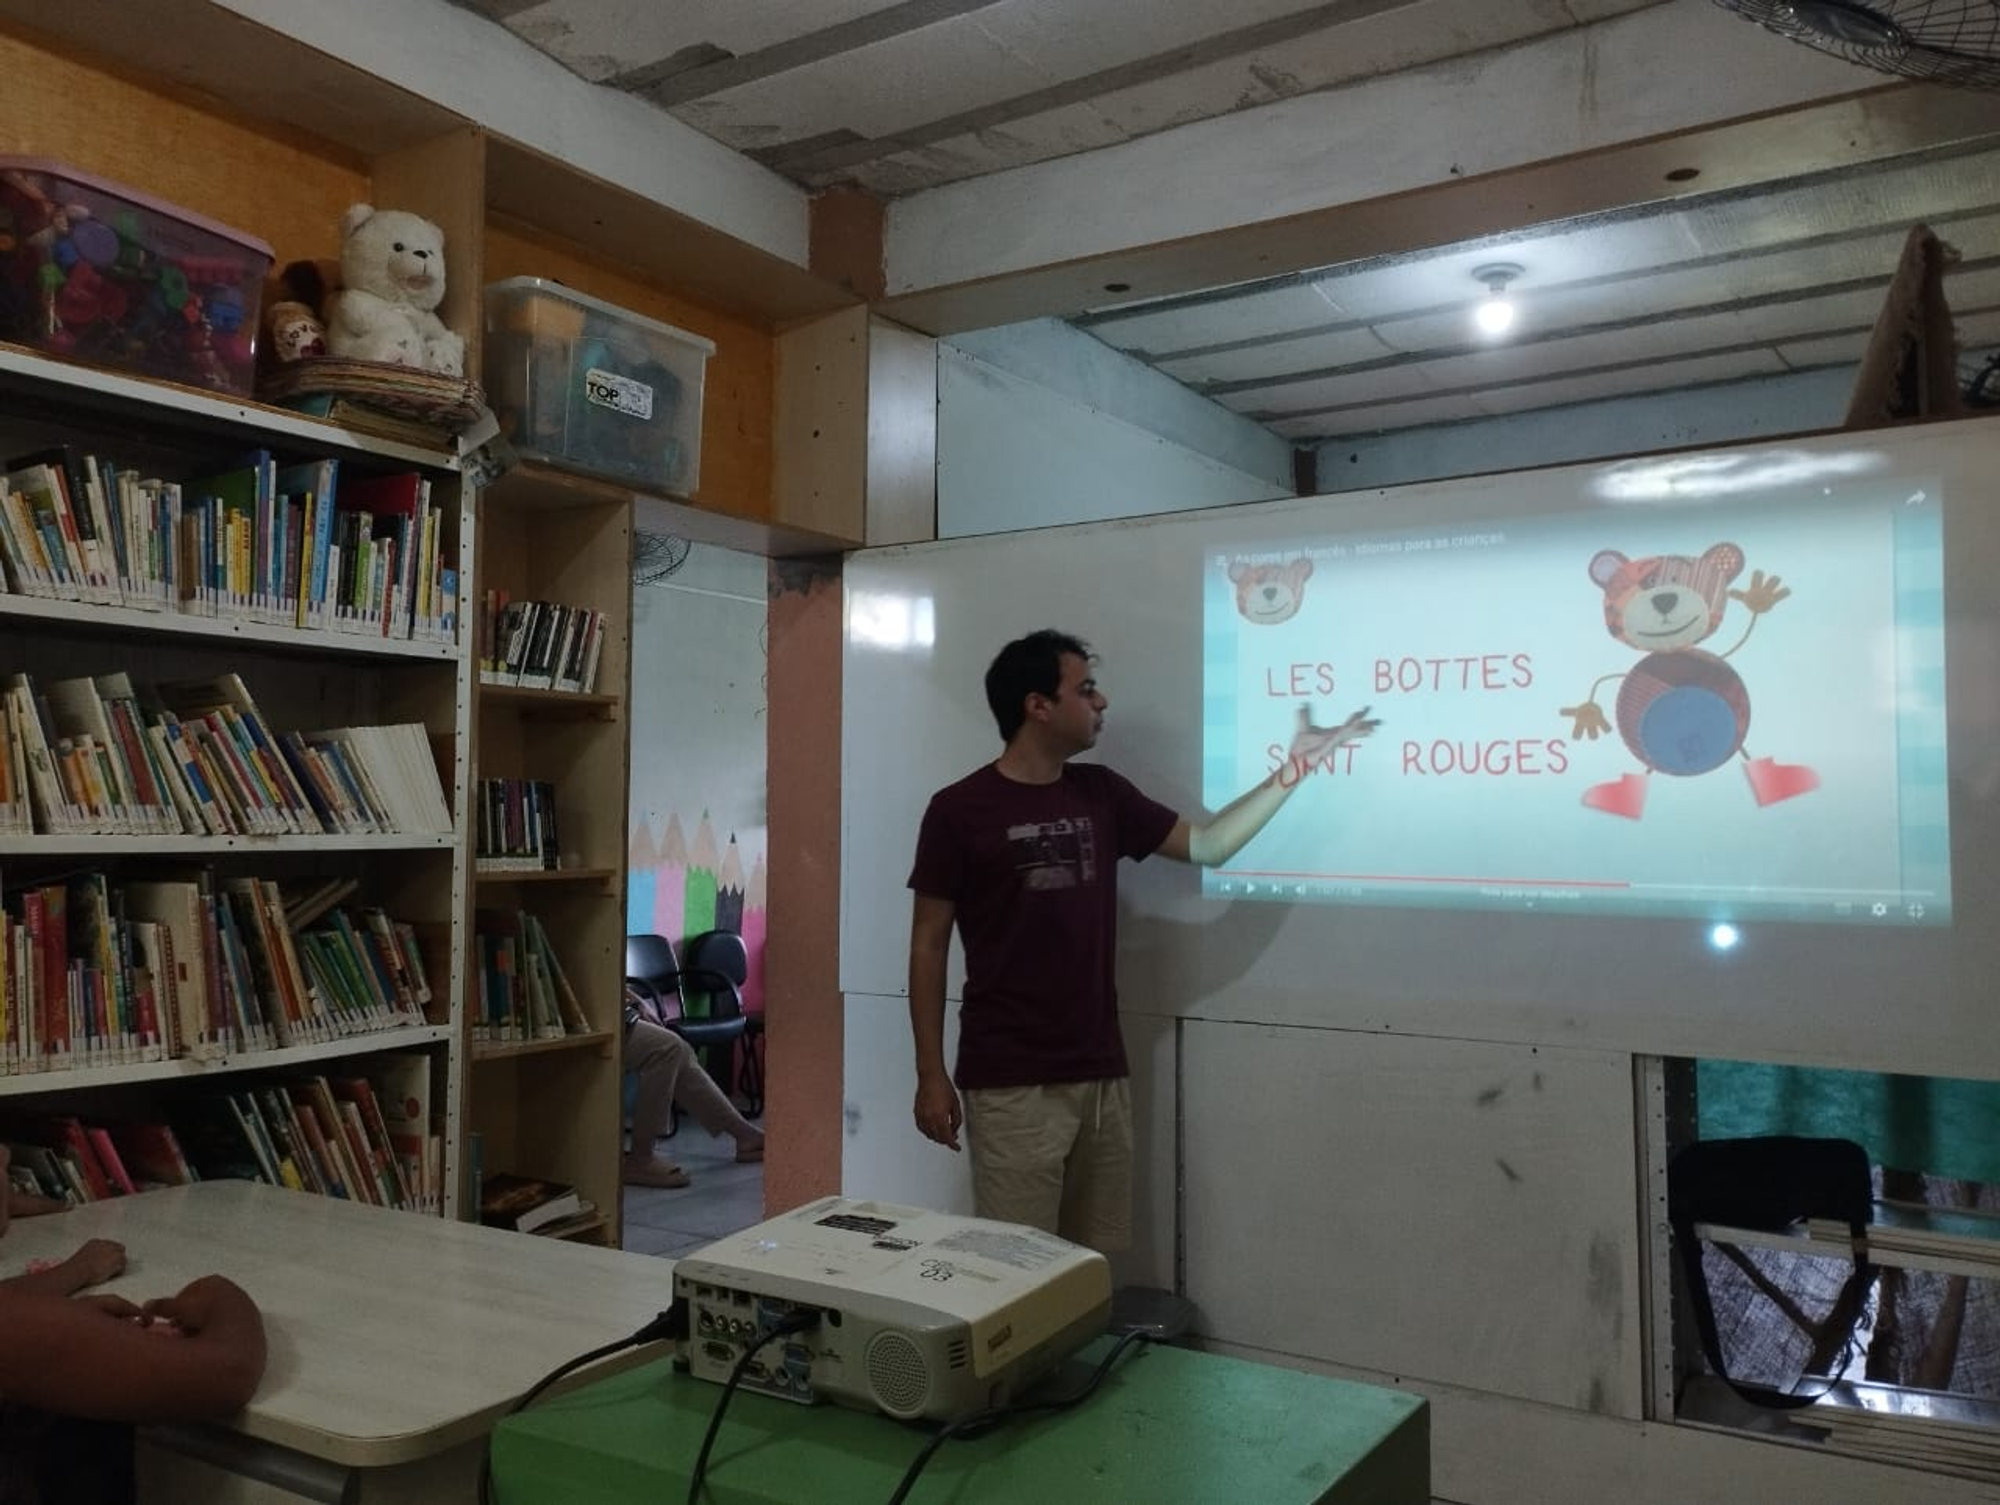
\includegraphics[width=0.5\textwidth]{imagem5.png}
    \caption{Foto 2 aula de francês}
    \label{fig:foto1505}
\end{figure}

\newpage

\subsubsection{Oficina de Origami}
Duas das três oficinas foram concluídas dentro do tempo previsto. No entanto, a primeira atividade excedeu o tempo planejado, interferindo no período reservado para a oficina de mágica. Todavia, as outras duas oficinas foram realizadas conforme o cronograma, proporcionando um excelente aprendizado e diversão para as crianças. Em todas as três atividades, as crianças se envolveram muito e adquiriram conhecimentos valiosos para levar para suas casas e para a vida. A seguir, os links dos vídeos usados e algumas fotos das atividades realizadas:

\vspace{1cm}

\href{https://youtu.be/pzS0ToWZ9DA?si=ObnPbtDY5x3C888C}{Vídeo de apoio 1 (Tsuru)}\\

\href{https://youtu.be/wMP6qhHYKFE?si=oCtZ1KJRkNBfFcck}{Vídeo de apoio 2 (Sapo)}\\

\begin{figure}[h]
    \centering
    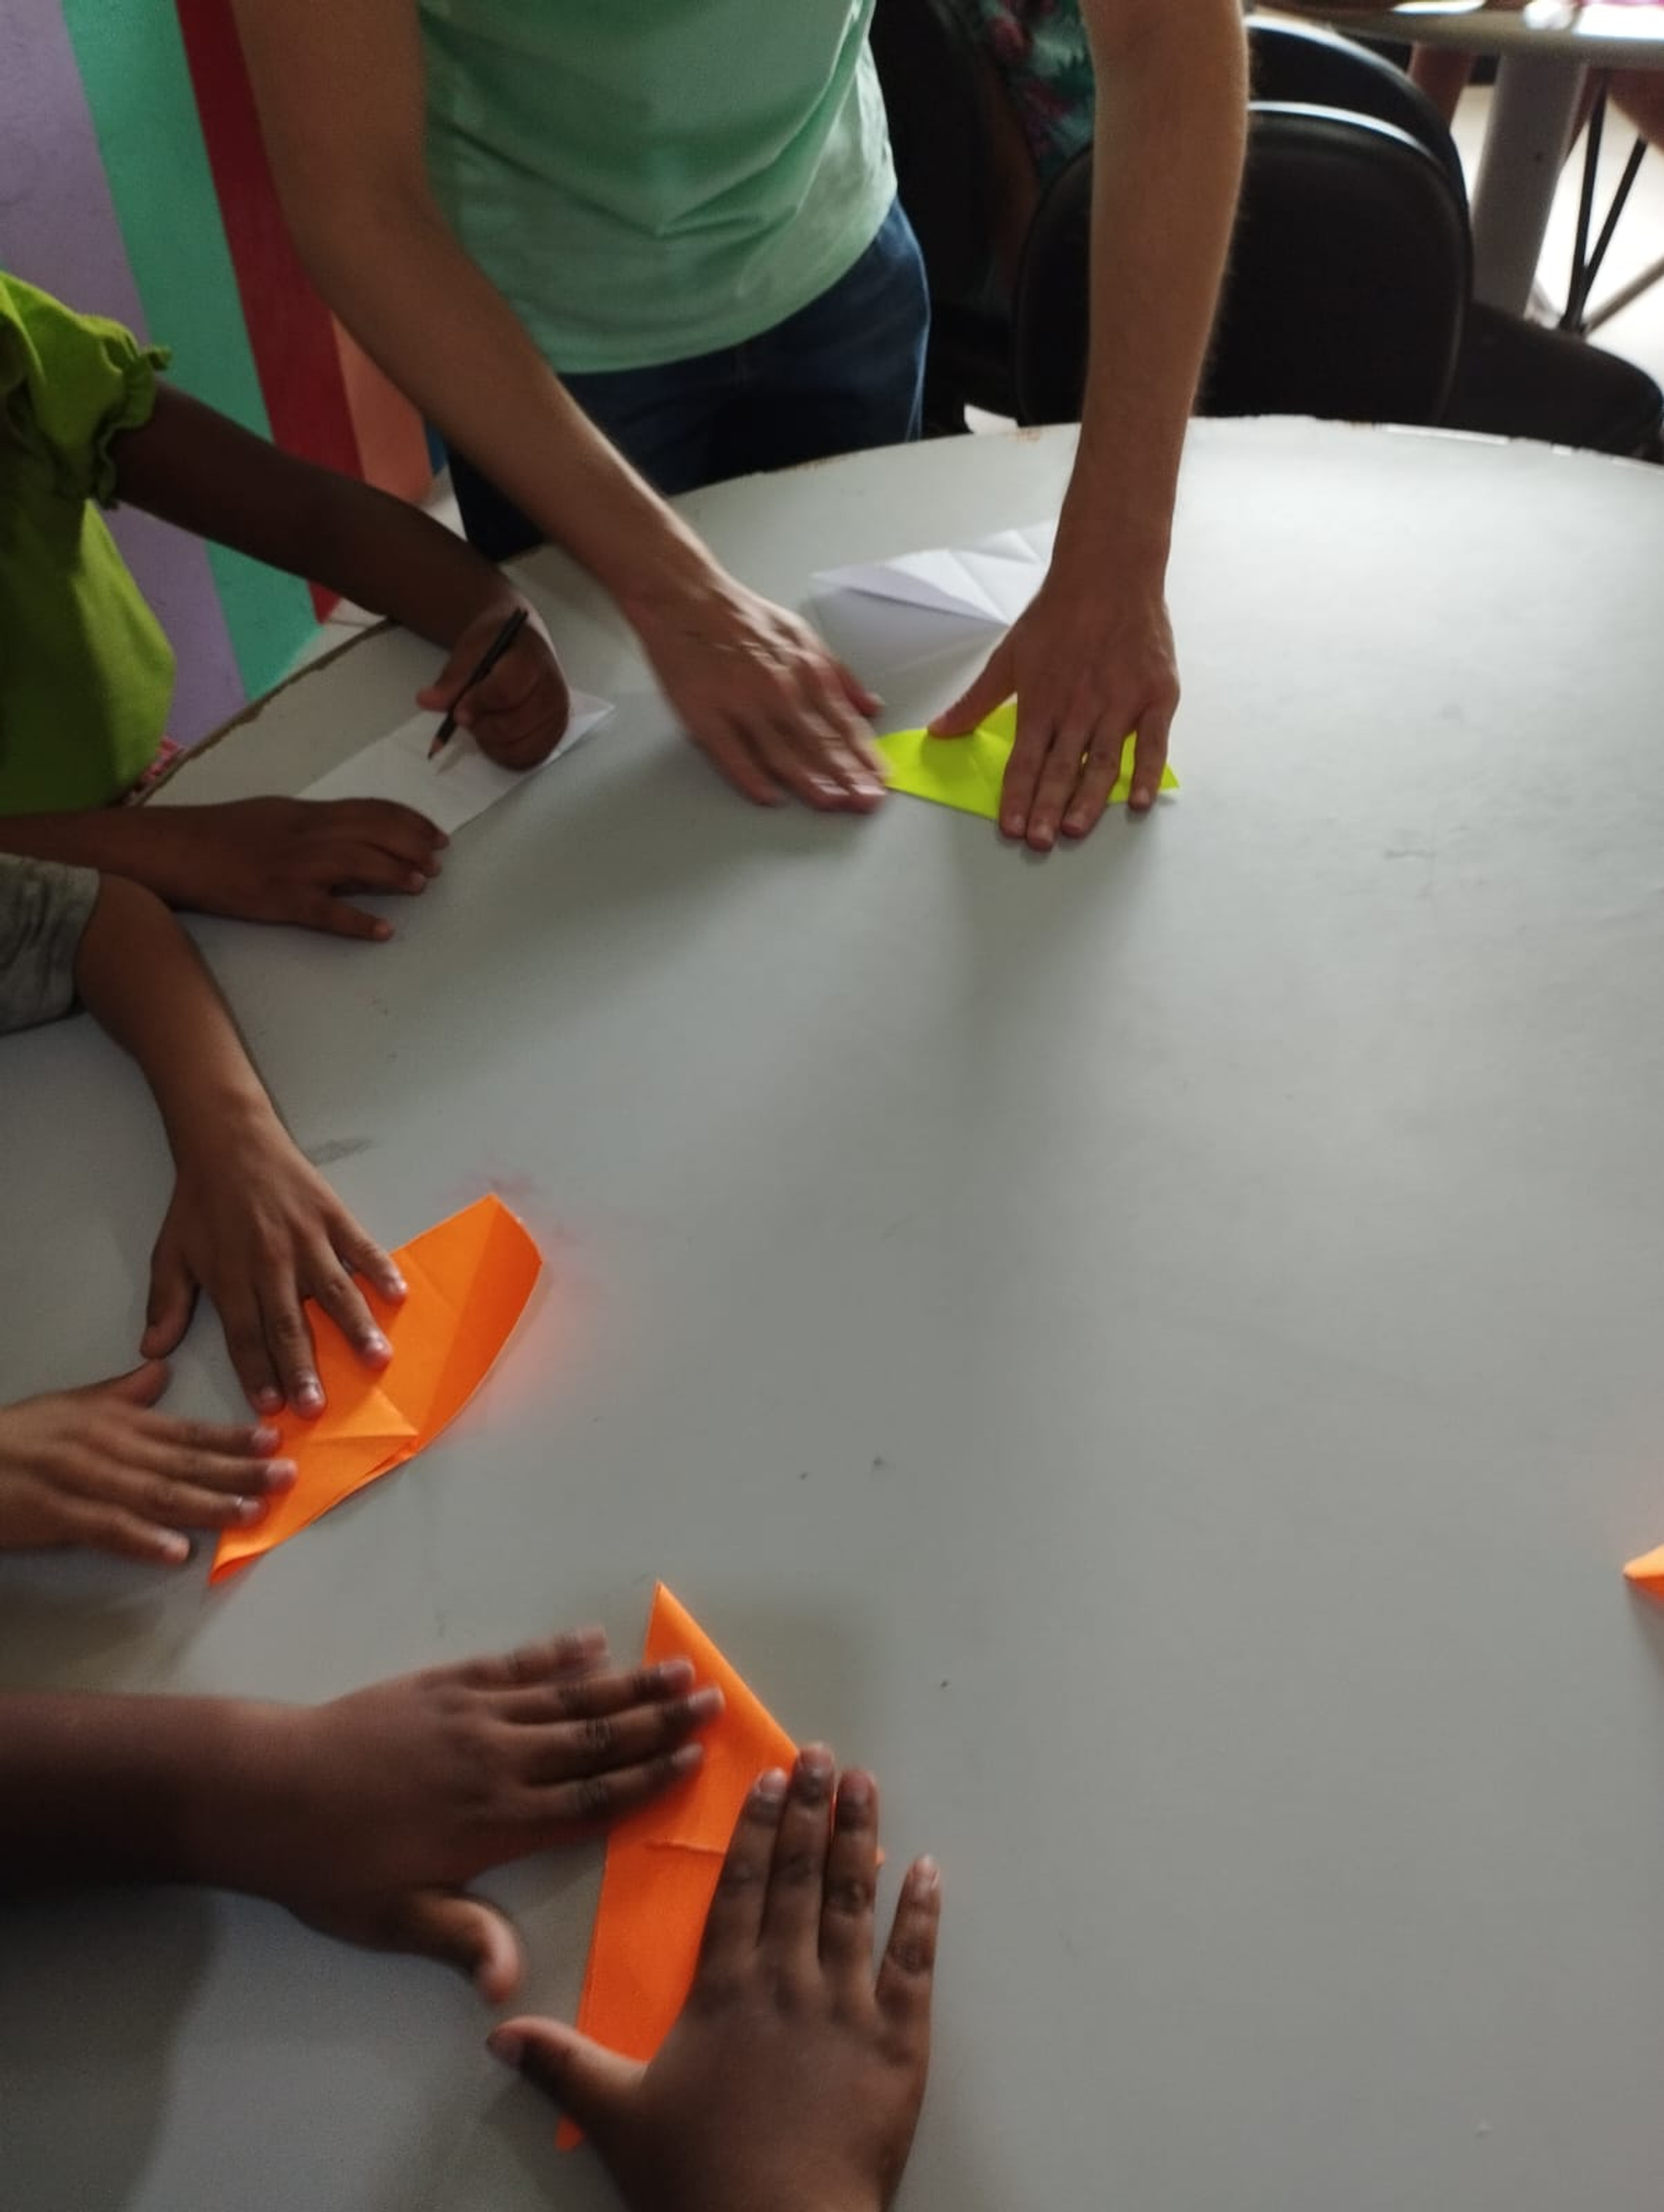
\includegraphics[width=0.5\textwidth]{imagem 6.png}
    \caption{Foto 1 oficina origami}
    \label{fig:foto1505}
\end{figure}

\vspace{1cm}

\begin{figure}[h]
    \centering
    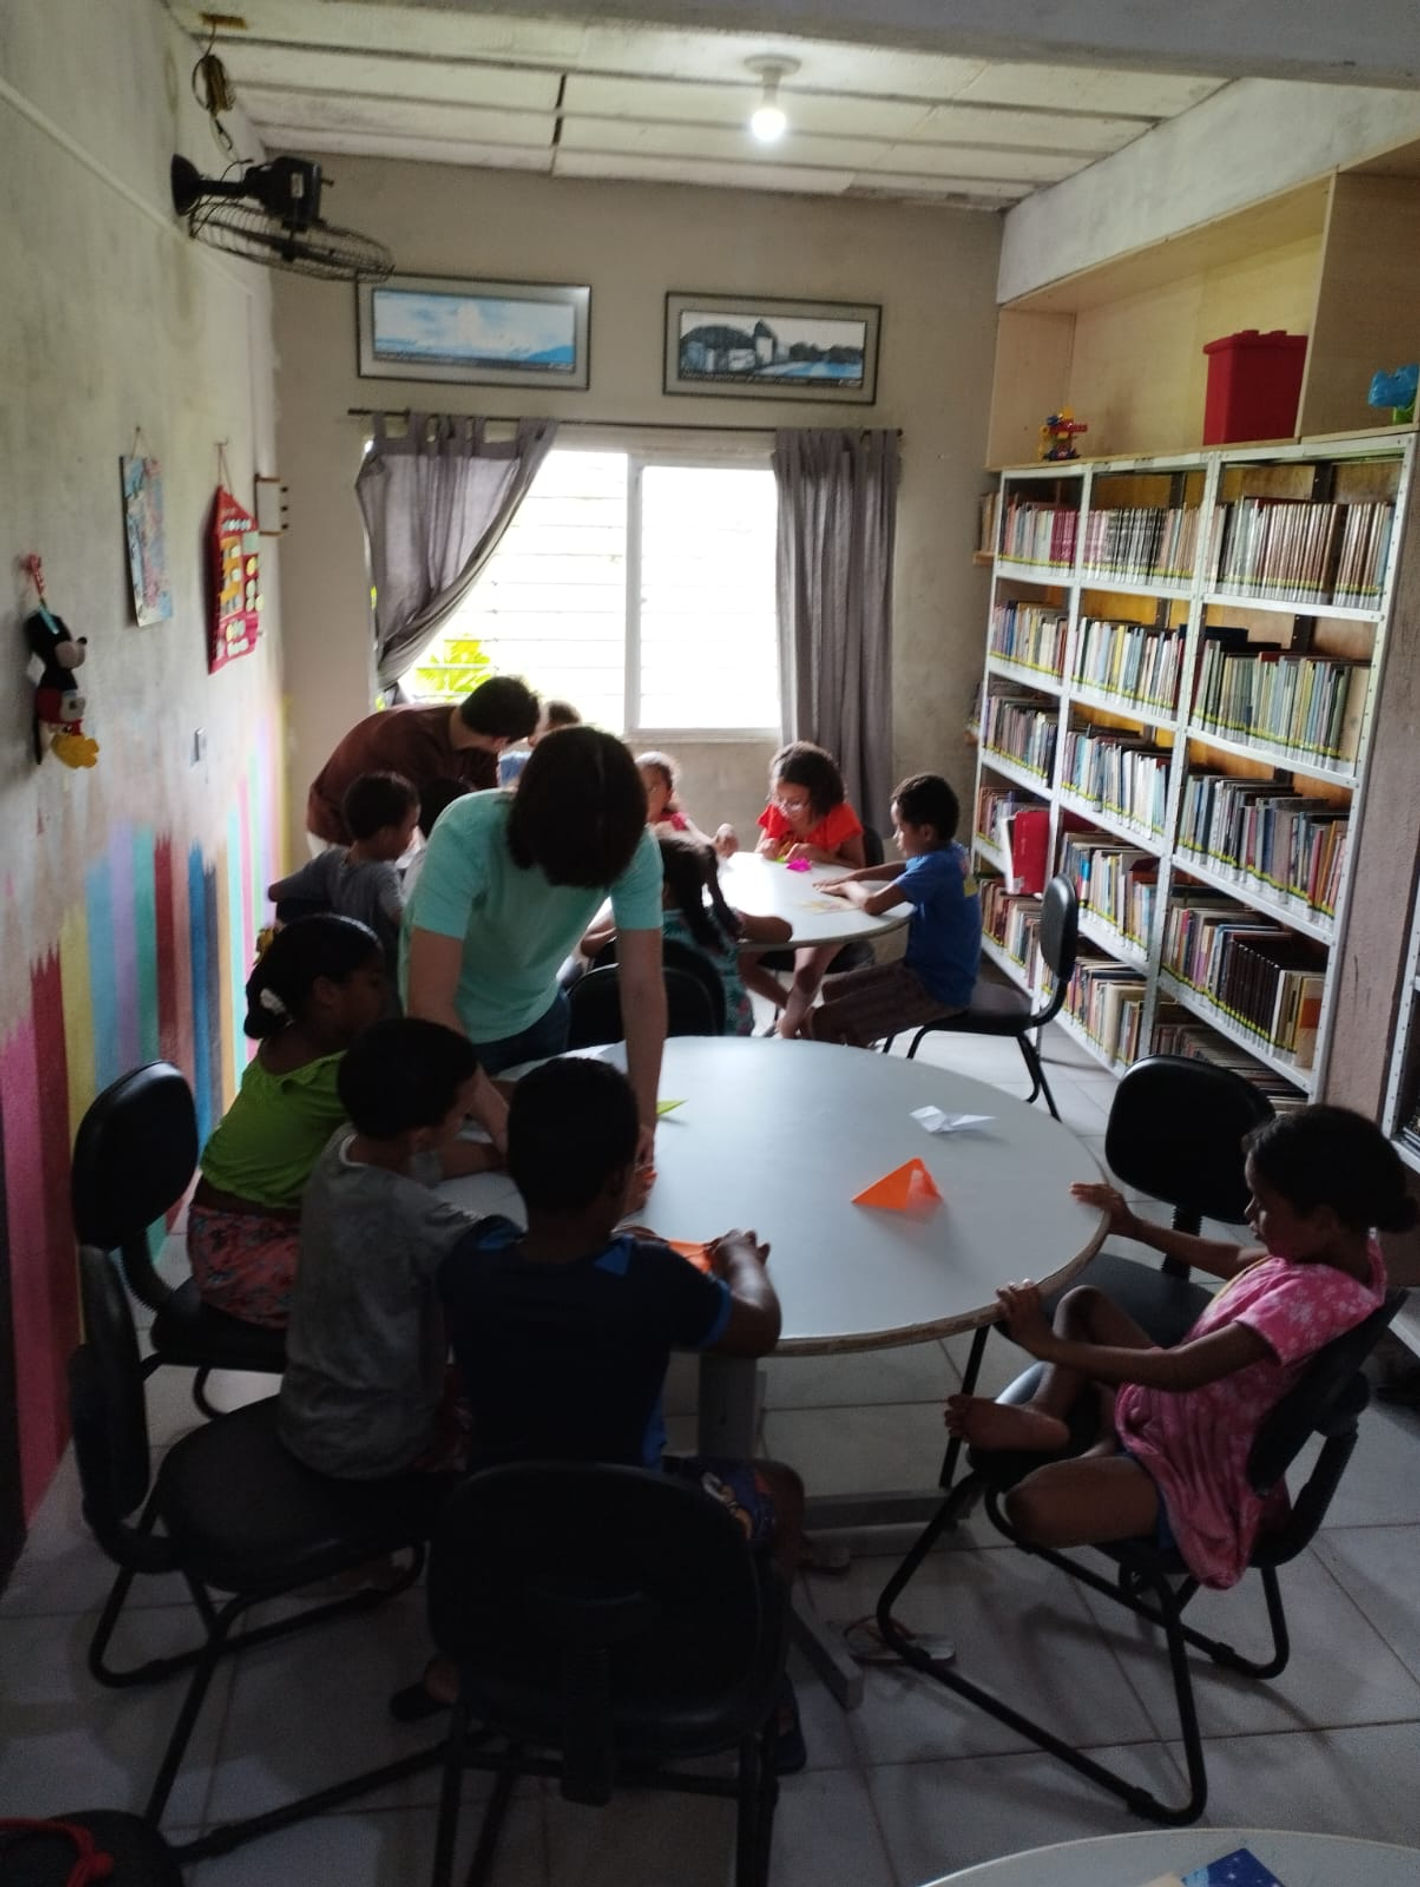
\includegraphics[width=0.5\textwidth]{imagem7.png}
    \caption{Foto 2 oficina origami}
    \label{fig:foto1505}
\end{figure}

\newpage

\subsubsection{Oficina de Mágica}
Infelizmente, não foi possível efetivar essa atividade. Devido ao atraso na primeira oficina de origami, agendada para o dia 17 de abril de 2024, das 9h20 às 10h20, a oficina de mágica ficou com menos de 40 minutos para ser realizada. Diante dessa situação, conversamos com o anfitrião, Reginaldo, e chegamos ao consenso de que seria melhor não realizar a atividade, pois os responsáveis viriam buscar as crianças em poucos minutos para que elas pudessem ir ao colégio. Consequentemente, não possuímos fotos ou registros dessa atividade.

\vspace{0.5cm}
\subsection{\Large{Discussão}}
Após a conclusão de todas as atividades, membros do grupo realizaram uma discussão abrangente sobre todo o trabalho realizado. Durante essa troca de ideias, surgiram pontos de destaque e conclusões significativas, as quais serão detalhadas no próximo tópico (6. Conclusão).

\newpage{}

\section{\LARGE{Conclusão}}
Conforme discutido no tópico (5.2. Discussão), ao término das atividades, os participantes que discutiram chegaram a uma conclusão relevante. Ficou nítido que simplesmente dialogar com as crianças não era suficiente para promover um crescimento saudável e o uso adequado das telas. Portanto, a decisão que foi tomada de implementar atividades lúdicas para estimular interesses por hobbies criativos se revelou ser uma abordagem significativamente mais eficaz quando o assunto é crescimento "sustentável", uma vez que as crianças se demonstraram muito entusiasmadas por todas as atividades propostas, destacando-se, em particular, a atividade da oficina de origami.\vspace{0.3cm}\\
Dessa maneira, concluíram-se as atividades da componente educacional da disciplina de Computação, Sociedade e Sustentabilidade. Levamos conosco todo o afeto e carinho manifestado pelas crianças da biblioteca, além da satisfação em saber que contribuímos, ainda que minimamente, para o desenvolvimento de cada uma delas. Estamos convictos de que essas interações deixarão uma marca inesquecivel em suas vidas, influenciando positivamente em seu crescimento e aprendizado.\vspace{0.3cm}\\\\ 

Ass: Nunno Wakiyama

\end{document}
